\chapter{Results}
\label{sec:results}
\subsection{Numerical experiments}

The charging behaviour of a spacecraft is dependent on several factors; the material composition of the craft, its dimensions, its location in space, the local time, and the space weather \parencite{LAI2019} \todo{Update reference, bib file contains extract of the book}. In this thesis, I wish to investigate what effects the presence of MMO's booms have on its charging behaviour, additionally I wished to investigate whether the direction of the ambient plasma drift or the photoelectron temperature would significantly change how the spacecraft charges.

The booms on the MMO extend the characteristic length of the spacecraft to be longer than that of the Debye length of the plasma found in table \ref{tab:PlasmaParamMMO}, as such I expect there to be a difference in the thickness of the plasma sheaths formed. 

Varying the direction of drift may impact the convection of photoelectron away from the surface of the sunlit surface of the spacecraft, which could potentially lead to a difference in the floating potential. Varying the average energy of the emitted photoelectrons will change the charging behaviour of the MMO, as seen in the Rosetta charging simulation paper \parencite{Sjogren2012}. To observe to what extent the floating potential and the thickness of the plasma sheath changes is the goal of varying the photoelectron temperature. 

\begin{center}
\begin{table}[H]
%\centering
\begin{tabular}{p{1.5cm}|p{1.5cm}|p{1.5cm}|p{1.5cm}|p{1.5cm}|p{1.5cm}|p{1.5cm}}
\toprule
\toprule
 & No photoelectrons & drift along $+X$ axis & drift along $-Z$ axis & Inclusion of booms & Mercury magnetic field & Photoelectron temp. $3 \; eV$ \\
\hline
Case 1 & \text{X} & \text{X} & & & &\\
\hline
Case 2 & & \text{X} & & & &\\
\hline
Case 3 & & & \text{X} & & &\\
\hline
Case 4 & & & \text{X} & & \text{X} &\\
\hline
Case 5 & & & \text{X} & & & \text{X}\\
\hline
Case 6 & \text{X} & \text{X} & & \text{X} & &\\
\hline
Case 7 & & \text{X} & & \text{X} & &\\
\hline
Case 8 & & & \text{X} & \text{X} & &\\
\hline
Case 9 & & & \text{X} & \text{X} & \text{X} &\\
\hline
Case 10 & & & \text{X} & \text{X} & & \text{X}\\
\bottomrule
\bottomrule
\end{tabular}
\caption{Summary of the numerical experiments of the MMO in orbit around Mercury, carried out with PINC}
\label{tab:MMOexperiments}
\end{table}
\end{center}

Table \ref{tab:MMOexperiments} gives an overview of the numerical simulations of the MMO spacecraft carried out for this thesis, case 1 and case 5 give a baseline of the charging behaviour where no photoemission is included and serves as a point of comparison between the photoelectron current and the ambient electron plasma current the MMO is subjected to. 

Cases 1 to 5, and cases 5 to 10 are equivalent but for the inclusion of the booms, with case 9 being the closest to the true conditions the MMO will experience when its orbit passes over the north cusp (ecliptic north) of Mercury. As such, case 8 is used as the baseline for the simulation in which the photoelectron temperature is varied from the value computed by PINC.

Save for cases 1 and 6, the simulations without photoemission, the computational domain was decomposed into 64 sub-domains for parallel processing. Cases 1 and 6 were decomposed into 128 sub-domains, the reason being that in the cases containing photoemission, the domain was not divided along the x-axis thus splitting the spacecraft in the YZ plane. This would account for another surface interior to the spacecraft that would have to be discarded as a source for photoemissive nodes.

For the sake of brevity, we will refer to the case number as shown in table \ref{tab:MMOexperiments} when presenting analyses for these five experiments. Results will be presented in order such that the plasma conditions closest to those the MMO will actually experience when orbiting the MMO is presented as the last simulation where photoemission parameters are computed directly. Photoemission with a different electron temperature is also presented, since an assumption of constant photoelectron yield was made, the impact of a higher photoelectron temperature will be compared to the other experiments in which the average photoelectron temperature was computed using Planck's law. We have also chosen to group simulations with and without booms together to make comparison across the two configurations simpler.

Save for a computational charging analysis of the combined bepiColombo spacecraft under thrust (using the MTM, the Mercury Transfer Module) \insertref{ESA Bepi sim} we were unable to find similar numerical experiments of the charging of the MMO spacecraft, we will therefore compare our results to theory through current balance analysis as presented in \ref{sec:theory}. As well as compare our results qualitatively to numerical charging experiments for different plasma parameters and different objects, such as in the paper by Deca et al. \parencite{Deca2013} used for our verification simulations.

From current balance, with photoemission included, we expect the variation of drift direction (comparing cases 2 and 3 to cases 7 and 8) to have minimal impact on the floating potential PINC will converge to, similarly we expect the sheath thickness and sheath plasma densities to be comparable for different drift directions. Across all five simulation types run, we expect the floating potential and sheath thickness to be larger in magnitude when the booms on the MMO are fully extended; since the booms are modeled as photoemissive, the greater surface area will lead to an overall higher electron current flowing from the spacecraft leading to a higher floating potential. 

The inclusion of the external magnetic field of Mercury could potentially impact the fraction of photoelectrons with a greater than average temperature being able to leave the surface of the spacecraft, if the particles' velocity vector does not align with the magnetic field the force exerted by the magnetic field could trap electrons more efficiently, leading to a lower floating potential.        

%FLOATING POTENTIAL SUMMARY
% \begin{table}[]
% \centering
% \begin{tabular}{cccccc}
% \hline
% & No photoelectron & Drift along Z & Drift along X & External Magnetic Field & Photoelectron temperature 3 eV\\\hline
% With booms & N/A & 105.419 & 105.400 & 105.400 & 78.154\\\hline
% Without booms & N/A & 100.710 & 100.696 & 100.699 & N/A\\\hline
% \end{tabular}
% \caption{Dummy text}
% \label{tab:FlotingPotSummary}
% \end{table}
\section{Charging without photoemission}
%FLOATING POTENTIAL CONVERGENCE
\begin{center}
    \begin{figure}[H]
      \begin{subfigure}[b]{0.75\textwidth}
      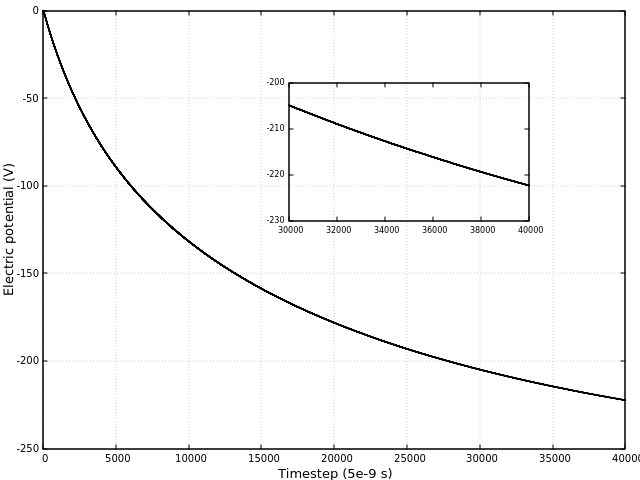
\includegraphics[width=\columnwidth]{figures/MMO/noPH/WB/C_noPH_WB.png}
      \caption{Booms}
      \label{fig:C_noPH_WB}
    \end{subfigure}
    \par\bigskip
    \begin{subfigure}[b]{0.75\textwidth}
      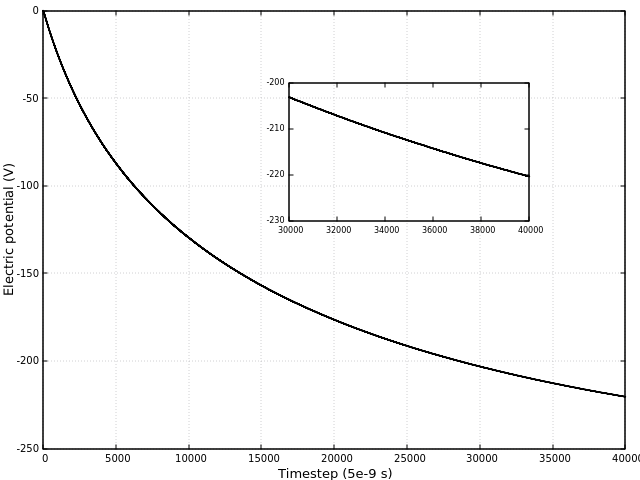
\includegraphics[width=\columnwidth]{figures/MMO/noPH/NB/C_noPH_NB.png}
      \caption{Without booms}
      \label{fig:C_noPH_NB}
    \end{subfigure}
  \caption{Timeseries plot of potential of the MMO with and without booms. The potential has been converted from PINC dimensionless units to Volts. The inset plots shows the potential of the two configurations for last 10,000 timesteps.}
    \label{fig:ConvnoPH}
  \end{figure}
\end{center}

The timeseries in fig \ref{fig:ConvnoPH} plots the potential of the MMO for each timestep simulated. From each inset plot, both for the MMO with booms and without, it is apparent from the slope that the system has not converged to a floating potential. Since the ambient plasma density around the MMO were approximately 100 times less dense than the value used in the verification simulation and no other current than ambient particle charging was present, a larger timestep was used in addition to a longer total simulation time. 

In order to compare our results with theory, we can estimate the floating potential the simulation would have converged to by fitting a function to our data and propagating the function forward in time until a steady state has been reached. Using Hill's function of the form 
\begin{equation*}
    \phi(t) = \phi_f \frac{t}{h + t},
\end{equation*}
where $\phi_f$ is the MMO floating potential without a photoemission current present, we estimate a floating potential of $\phi_f \approx 283 V$. A full analysis of the curve fitting and the Python script used to fit the curves is given in  \cref{sec:appendixC}, and a current balance analysis of the theoretical floating potential for the boomless configurations of the MMO (with and without the photoemission current) will be presented in the impending section. 


%POTENTIAL THROUGH CENTER OF OBJECT
\begin{center}
    \begin{figure}[H]
      \begin{subfigure}[b]{0.61\textwidth}
      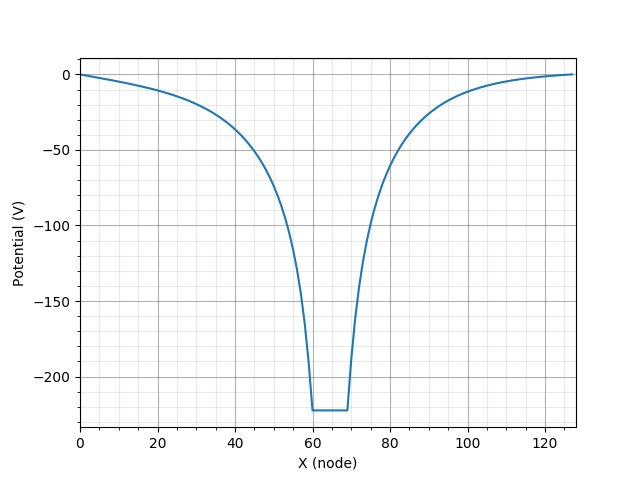
\includegraphics[width=\textwidth]{figures/MMO/noPH/WB/L_noPH_WB.png}
      \caption{Booms}
      \label{fig:L_noPH_WB}
    \end{subfigure}
    \begin{subfigure}[b]{0.61\textwidth}
      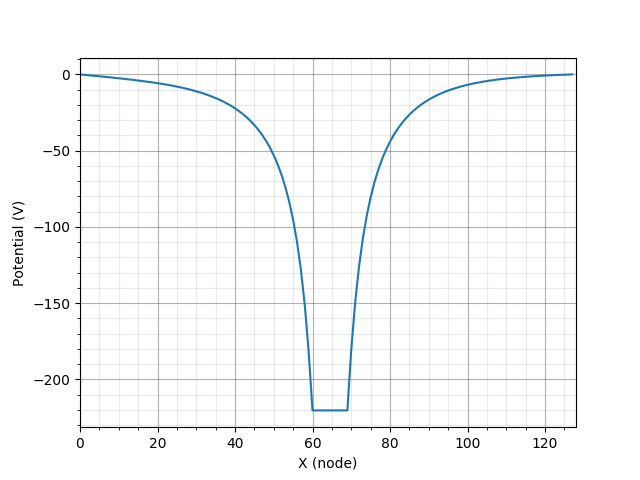
\includegraphics[width=\textwidth]{figures/MMO/noPH/NB/L_noPH_NB.png}
      \caption{Without booms}
      \label{fig:L_noPH_NB}
    \end{subfigure}
  \caption{\ref{fig:L_noPH_NB} and \ref{fig:L_noPH_WB} show a potential profile along the X axis for the MMO without and with booms respectively. The line is plotted at $(x,y) = (13.95 m, 13.95 m)$, or node points $(x,y) = (62,62)$, and passes through the main octagonal body of the spacecraft. The X axis units are in number of nodes from the origin.}
\label{fig:Line_noPH_comb}
  \end{figure}
\end{center}

Even without PINC converging to a floating potential, we can still make comparisons of the plasma sheath formed around the spacecraft by plotting the potential profile of the domain. Figure \ref{fig:Line_noPH_comb}, shows the potential relative to the ambient plasma plotted on a center line passing through the spacecraft octahedral body. comparing figure \ref{fig:L_noPH_WB} with figure \ref{fig:L_noPH_NB}, we see a difference in sheath thickness. For a negatively charged probe, we can estimate the thickness of the sheath using Bohm's sheath criterion \parencite{Chen2018}:
\begin{equation}
    u_0 \approx \left(\frac{K T_e}{m_i}\right)^{1/2},
\end{equation}
where $u_0$ is the velocity required by ions at the sheath boundary. For ions to be accelerated to this velocity we can estimate the required sheath edge potential as
\begin{equation}
    \phi_s = -\frac{1}{2} \frac{K T_e}{e}.
\end{equation}

Where $\phi_s$ is the potential relative to the ambient plasma. Setting the electron temperature, $T_e$, to $1.16 \times 10^6$ we find the sheath boundary potential to be approximately $-50 V$ relative to the main plasma body. The sheath thickness is then the distance from the potential along the x axis to where the potential is the same as the sheath boundary potential. From the plots we then estimate a sheath thickness of 2.5 meters for the MMO configuration without booms, and 3.2 meters for the configuration with booms.

The sheath thickness, $d$, can also be computed directly by re-arranging the Child-Langmuir law \parencite{Chen2018}:
\begin{equation}
    d^2 = \frac{4}{9} \left(\frac{2e}{m_i}\right)^{1/2} \frac{\abs{\phi_w}^{3/2}}{4 \pi \abs{\vb{j_{i,s}}}}.
\end{equation}
where $\phi_w$ is the "wall", or spacecraft potential, and $\abs{\vb{j_{i,s}}}$ is the ion saturation current density. The ion saturation current density is given by
\begin{equation}
    \abs{\vb{j_{i,s}}} = q_e n_e c_s.
\end{equation}
The speed $c_s$ is the ion speed of sound, and can be estimated as $c_s = \sqrt{k_b T_e / m_i}$ for a cold plasma. These equations are straight forward to solve by plugging in the known spacecraft potential, the electron density, and electron temperature. Using the parameters from table \ref{tab:PlasmaParamMMO}  the plasma thickness comes out to be 3.13 meters. 

%AVERAGE POTENTIAL ISOLINES XY
\begin{center}
\begin{figure}[hb!]
  \begin{subfigure}[b]{0.61\textwidth}
    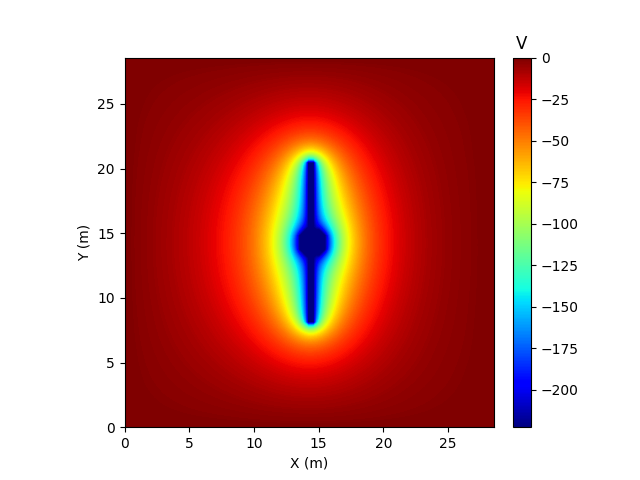
\includegraphics[width=\textwidth]{figures/MMO/noPH/WB/P_noPH_WB.png}
    \caption{Booms}
    \label{fig:P_noPH_WB}
  \end{subfigure}
  \hfill
  \begin{subfigure}[b]{0.61\textwidth}
    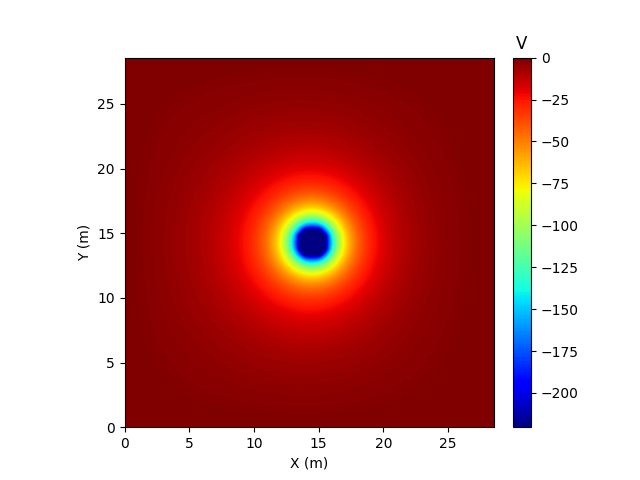
\includegraphics[width=\textwidth]{figures/MMO/noPH/NB/P_noPH_NB.png}
    \caption{Without booms}
    \label{fig:P_noPH_NB}
  \end{subfigure}
  \caption{\ref{fig:P_noPH_WB} and \ref{fig:P_noPH_WB} are 2D slices through $Z = 14.4 m$ showing the potential profile of the entire computational domain.}    \label{fig:PMMOnoPH}
\end{figure}
\end{center}

Figure \ref{fig:PMMOnoPH} shows 2D cut in the plane $Z=14.4$, dividing the spacecraft in half, and is plotted at the last simulated timestep (timestep 40,000). The contours are plotted using the matplotlib Python package, with contour lines subdivided into 500 levels to better distinguish the plasma sheath. Values are converted from normalized PINC internal values to Volts. The color boundary between orange and red approximately marks the plasma sheath edge. We can see this boundary is equidistant from the MMO body in the boomless configuration, whereas the sheath boundary is relatively closer to the boom tips than to the main octagonal body of the spacecraft. 

%PARTICLE DENSITIES (rho_i and rho_e)
%RHO_I
\begin{center}
    \begin{figure}[H]
      \begin{subfigure}[b]{0.61\textwidth}
      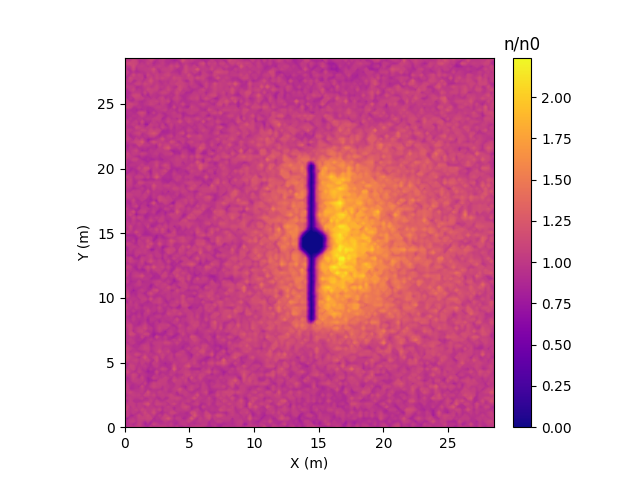
\includegraphics[width=\textwidth]{figures/MMO/noPH/WB/I_noPH_WB.png}
      \caption{Booms}
      \label{fig:I_noPH_WB}
    \end{subfigure}
    \begin{subfigure}[b]{0.61\textwidth}
      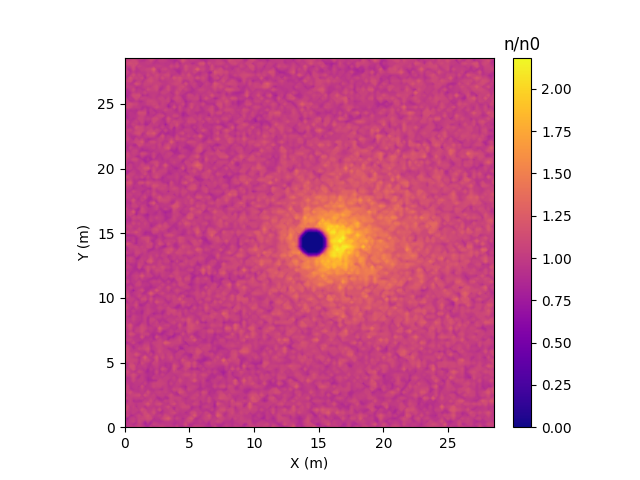
\includegraphics[width=\textwidth]{figures/MMO/noPH/NB/I_noPH_NB.png}
      \caption{Without booms}
      \label{fig:I_noPH_NB}
    \end{subfigure}
  \caption{Ion density profile plotted at $Z = 14.4 m$, the color gradient is normalized against the ion plasma density from table \ref{tab:PlasmaParamMMO}.}
\label{fig:IonsNoPH}
  \end{figure}
\end{center}

%RHO_E
\begin{center}
    \begin{figure}[H]
      \begin{subfigure}[b]{0.61\textwidth}
      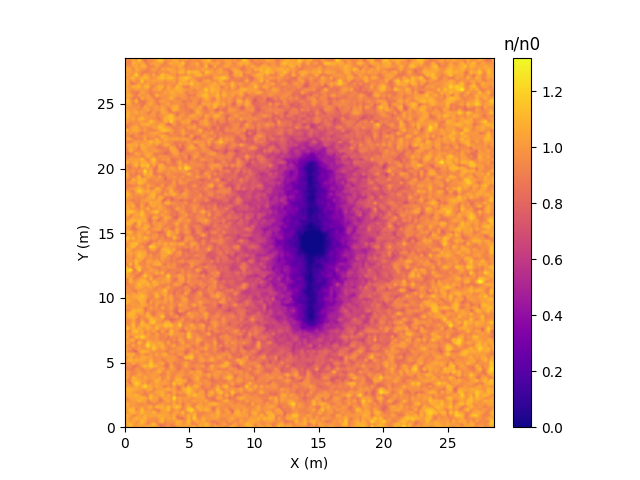
\includegraphics[width=\textwidth]{figures/MMO/noPH/WB/E_noPH_WB.png}
      \caption{Booms}
      \label{fig:E_noPH_WB}
    \end{subfigure}
    \begin{subfigure}[b]{0.61\textwidth}
      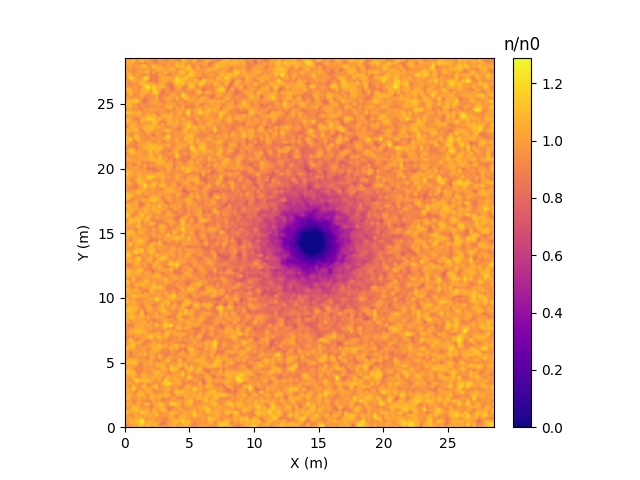
\includegraphics[width=\textwidth]{figures/MMO/noPH/NB/E_noPH_NB.png}
      \caption{Without booms}
      \label{fig:E_noPH_NB}
    \end{subfigure}
  \caption{Electron density profile plotted at $Z = 14.4 m$, the color gradient is normalized against the electron plasma density from table \ref{tab:PlasmaParamMMO}.}
  \label{fig:ElectronsNoPH}
  \end{figure}
\end{center}

Figures \ref{fig:IonsNoPH} and \ref{fig:ElectronsNoPH} show the density of ions (protons) and electrons respectively plotted at timestep 400, 1\% through the total simulation time. Similarly to figure \ref{fig:PMMOnoPH}, the 2D slice is placed at $Z = 14.4 m$, dividing the spacecraft in halves. The density values have been normalized against the ambient plasma density, and as before, 500 levels were used for the contour lines drawn. For cases 1 and 6, we set the plasma drift along the positive X axis, \ref{fig:IonsNoPH} clearly shows an ion wake forming "behind" the spacecraft for both boom configurations. We also note the slightly higher density of ions directly in "front" of the spacecraft, denoting the plasma sheath that has formed even this early in the simulation. Figure \ref{fig:ElectronsNoPH} gives the clearest picture of the shape of the plasma sheath formed around the spacecraft, in the MMO configuration with booms, the sheath forms an ellipsoid around the spacecraft where, relative to the ambient plasma, almost no electrons reside. The sheath in the boomless MMO configuration is circular in shape, which gives a good indication that computing the theoretical floating potential of the boomless MMO configuration can be done by assuming the MMO to be a cylinder with the same radius as the circle circumscribing the MMO octagonal body.

\section{Charging with photoemission}

\subsection*{Drift parallel to X axis}

%FLOATING POTENTIAL CONVERGENCE
\begin{figure}[H]
  \centering
  \begin{subfigure}[b]{0.75\textwidth}
  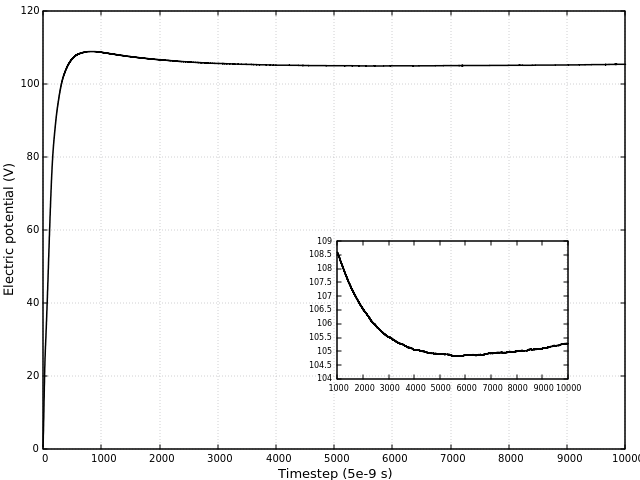
\includegraphics[width=\columnwidth]{figures/MMO/posX/WB/C_posX_WB.png}
  \caption{Booms}
  \label{fig:C_posX_WB}
\end{subfigure}
\hfill
\begin{subfigure}[b]{0.75\textwidth}
  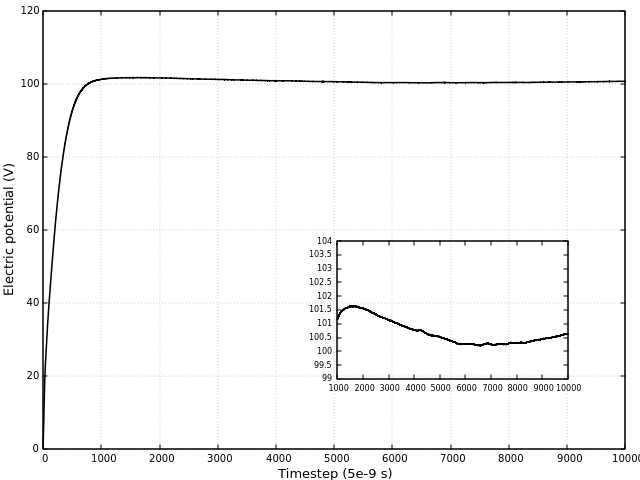
\includegraphics[width=\columnwidth]{figures/MMO/posX/NB/C_posX_NB.png}
  \caption{Without booms}
  \label{fig:C_posX_NB}
\end{subfigure}
\caption{Time series plot of the potential of the two MMO configurations for drift along X axis. The insets plots the same timeseries starting at 1000 timesteps, where the potential of the spacecraft has begun to oscillate about the floating potential.}
\label{fig:Conv_posX}
\end{figure}

Figure \ref{fig_Pot_posX} shows the convergence to the floating potential of both MMO configurations. Unlike the numerical simulations without photoemission, the potential of both configurations of the MMO converge rapidly to a its floating potential. The slope of the increase in potential early on in the simulation points to the high ratio between the photoemission current and the charging from the impinging electrons from the ambient plasma. The floating potential for MMO with booms, as seen in figure \ref{fig:P_posX_WB} overshoots the floating potential by several volts, before converging to 105.4 V. In the boomless configuration, figure \ref{fig:P_posX_NB}, the overshoot is much smaller, and the potential shows oscillatory behaviour around a floating potential of 100.7 V. The overshoot in the floating potential could result from the thin booms extending far from the main body of the MMO developing a potential barrier slower, and smaller in height, than the central body leading to a gradual rather than sudden decrease in the effective photoemission current.

%POTENTIAL THROUGH CENTER OF OBJECT

\begin{figure}[H]
  \begin{subfigure}[b]{0.6\textwidth}
  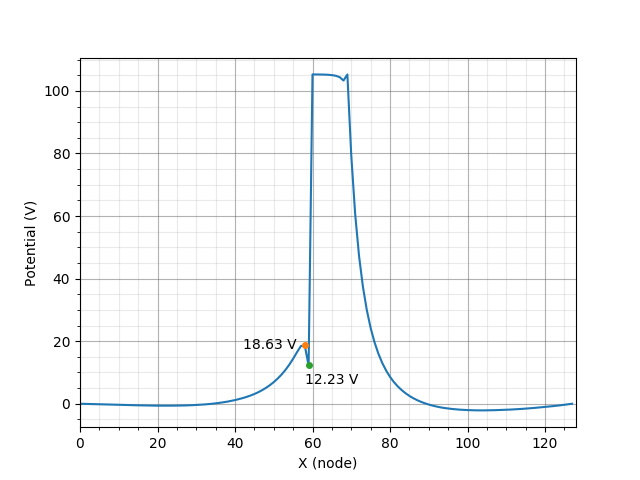
\includegraphics[width=\textwidth]{figures/MMO/posX/WB/L_posX_WB.png}
  \caption{Booms}
  \label{fig:L_posX_WB}
\end{subfigure}
\begin{subfigure}[b]{0.6\textwidth}
  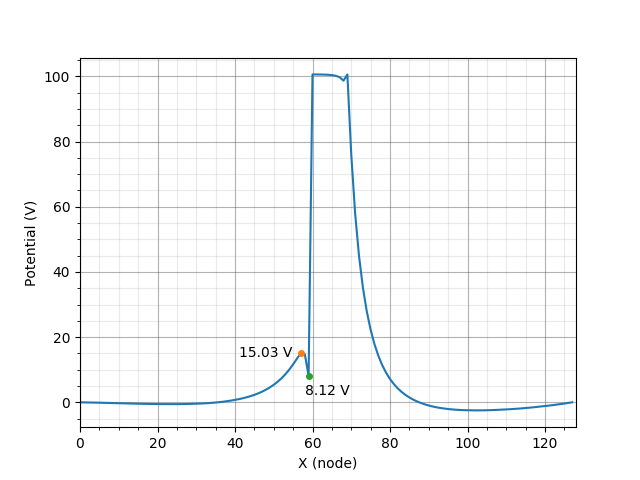
\includegraphics[width=\textwidth]{figures/MMO/posX/NB/L_posX_NB.png}
  \caption{Without booms}
  \label{fig:L_posX_NB}
\end{subfigure}
\caption{Potential profile along the X axis for the two MMO configurations with drift along the X axis and photoemission included. The line is plotted at $(x,y) = (13.95 m, 13.95 m)$, or node points $(x,y) = (62,62)$, and passes through the main octagonal body of the spacecraft. The X axis units are in number of nodes from the origin. The two values in each plot show the height of the potential barrier formed.}
\label{fig:Line_posX}
\end{figure}


%AVERAGE POTENTIAL ISOLINES XY

\begin{figure}[H]
  \begin{subfigure}[b]{0.6\textwidth}
    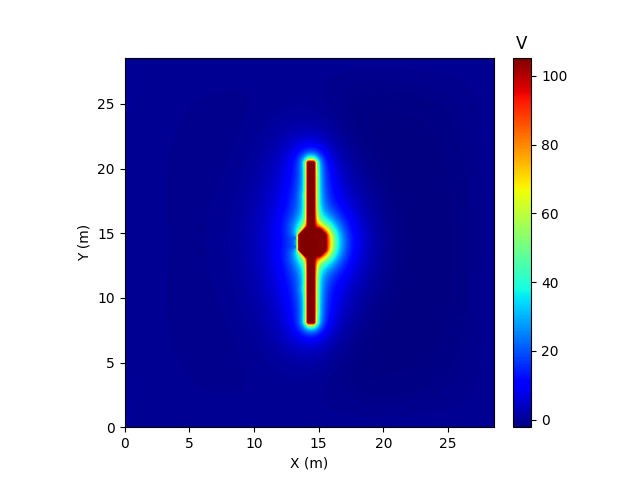
\includegraphics[width=\textwidth]{figures/MMO/posX/WB/P_posX_WB.png}
    \caption{Booms}
    \label{fig:P_posX_WB}
  \end{subfigure}
  \begin{subfigure}[b]{0.6\textwidth}
    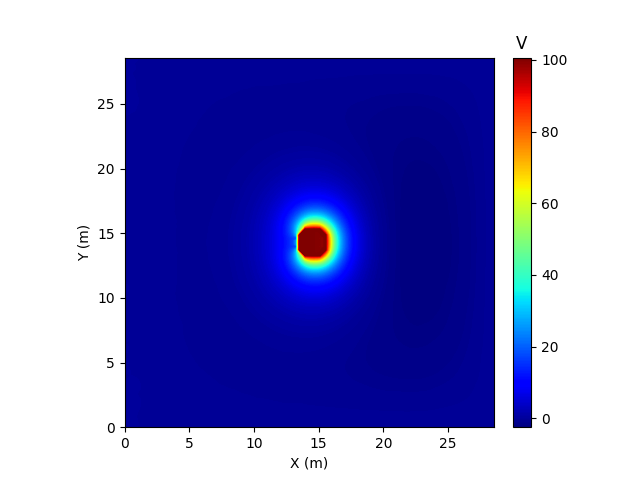
\includegraphics[width=\textwidth]{figures/MMO/posX/NB/P_posX_NB.png}
    \caption{Without booms}
    \label{fig:P_posX_NB}
  \end{subfigure}
  \caption{2D slices through $Z = 14.4 m$ showing the time averaged potential profile of the entire computational domain with drift along X axis, and photoemission included. The potential is time averaged after a floating potential has been reached after 1,000 timesteps.}
  \label{fig:Pot_posX}
\end{figure}



%PARTICLE DENSITIES (rho_i and rho_e)
%RHO_I

\begin{figure}[H]
  \begin{subfigure}[b]{0.6\textwidth}
  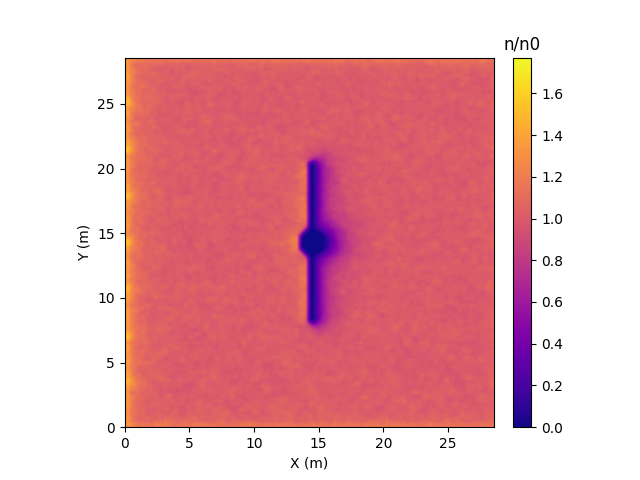
\includegraphics[width=\textwidth]{figures/MMO/posX/WB/I_posX_WB.png}
  \caption{Booms}
  \label{fig:I_posX_WB}
  \end{subfigure}
\begin{subfigure}[b]{0.6\textwidth}
  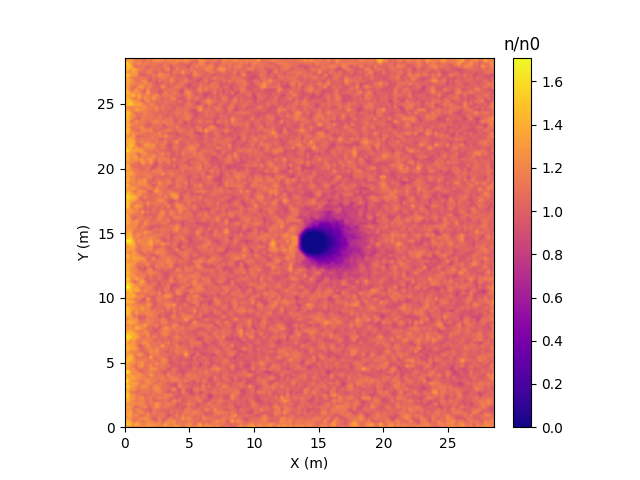
\includegraphics[width=\textwidth]{figures/MMO/posX/NB/I_posX_NB.png}
  \caption{Without booms}
  \label{fig:I_posX_NB}
\end{subfigure}
\caption{Ion density profile plotted at $Z = 14.4 m$, the color gradient is normalized against the ion plasma density from table \ref{tab:PlasmaParamMMO}. Plasma drift is along the X axis, and photoemission is included}
\label{fig:Ions_posX}
\end{figure}


%RHO_E

\begin{figure}[H]
  \begin{subfigure}[b]{0.6\textwidth}
  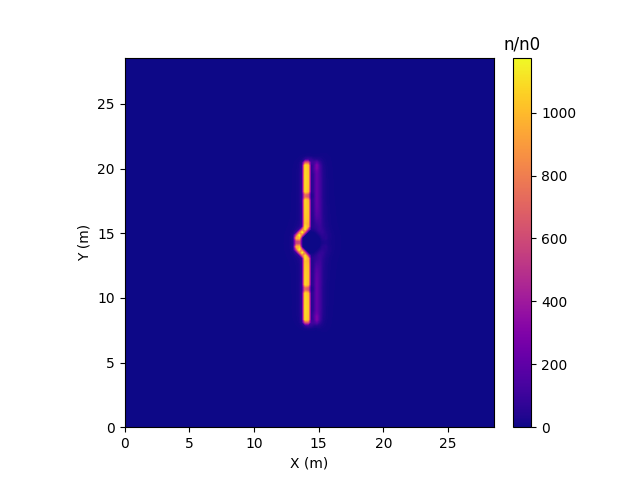
\includegraphics[width=\textwidth]{figures/MMO/posX/WB/E_posX_WB.png}
  \caption{Booms}
  \label{fig:E_posX_WB}
\end{subfigure}
\begin{subfigure}[b]{0.6\textwidth}
  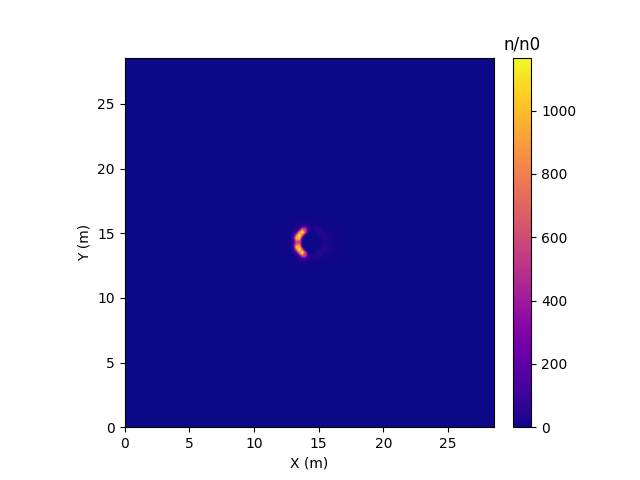
\includegraphics[width=\textwidth]{figures/MMO/posX/NB/E_posX_NB.png}
  \caption{Without booms}
  \label{fig:E_posX_NB}
\end{subfigure}
\caption{Electron density profile plotted at $Z = 14.4 m$, the color gradient is normalized against the electron plasma density from table \ref{tab:PlasmaParamMMO}. Drift is along the X axis, and photoemission is included, the sun is located in the negative X direction.}
\label{fig:Electrons_posX}
\end{figure}


Plasma particle densities are plotted for both ions (protons) and electrons in figures \ref{fig:Ions_posX} and \ref{fig:Electrons_posX} respectively. Due to a high photoemission current, the positively charged spacecraft does not form an ion wake, as can be seen in both \ref{fig:I_posX_WB} and \ref{fig:I_posX_WB}. Downstream of the spacecraft, there is a relative low ion density relative to the ambient plasma which is more prominent in the case of the boomless configuration of the MMO. When the electron density is restricted in figures \ref{fig:E_posX_WB} and \ref{fig:E_posX_NB} it can be seen that an electron wake forms behind the spacecraft instead. Without restriction in the maximum value of the contour lines, figures \ref{fig:E_posX_WB} and \ref{fig:E_posX_NB} show high concentration of electrons adjacent to the sunlit surfaces of the MMO, with electron densities as high as 1175 times the density of electrons in the ambient plasma. 

At such high densities, the local Debye length is significantly shorter than that of the ambient plasma. We can compute the local Debye length from equation \eqref{eq:Debyelength} and from the photoelectron temperature. The photoelectron temperature is computed in PINC internally by numerical integration of equation \eqref{eq:PlanckSum} in terms of energy and photons per second, subtracting the work function of the surface material gives the photoelectron temperature of $0.62 eV$. Substituting the photoelectron density and temperature into equation \eqref{eq:Debyelength} we have a local Debye length of only 0.017 meters.

\subsection*{Drift parallel to Z axis}
%FLOATING POTENTIAL CONVERGENCE

\begin{figure}[H]
  \centering
  \begin{subfigure}[b]{0.75\textwidth}
  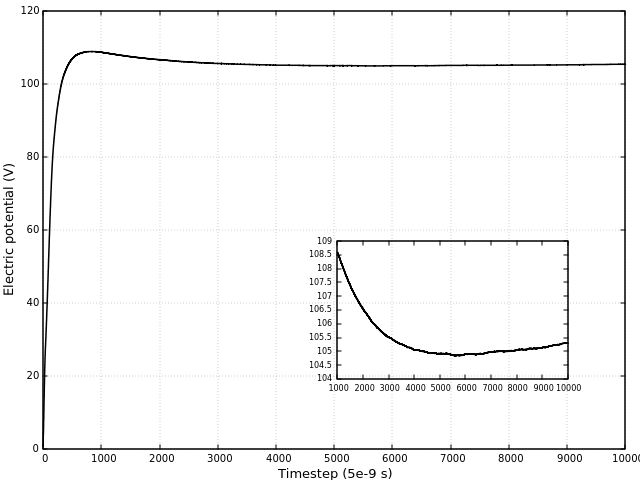
\includegraphics[width=\columnwidth]{figures/MMO/minZ/WB/C_minZ_WB.png}
  \caption{Booms}
  \label{fig:C_minZ_WB}
\end{subfigure}
\par\bigskip
\begin{subfigure}[b]{0.75\textwidth}
  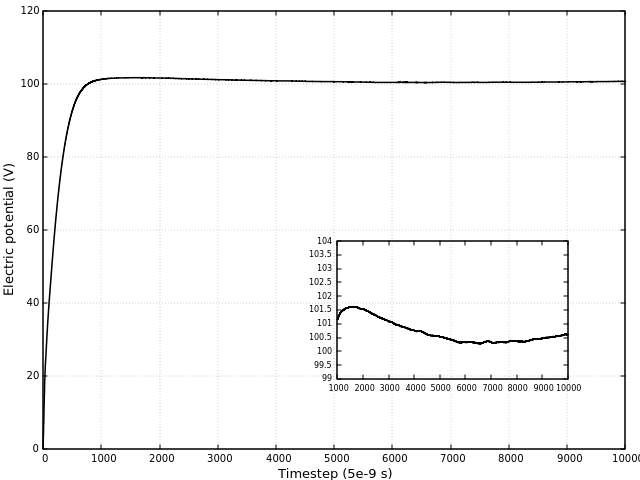
\includegraphics[width=\columnwidth]{figures/MMO/minZ/NB/C_minZ_NB.png}
  \caption{Without booms}
  \label{fig:C_minZ_NB}
\end{subfigure}
\label{fig:Conv_minZ}
\caption{Time series plot of the potential of the MMO with and without booms, where the drift is along the negative Z axis and photoemission is included. The inset plots the same timeseries after 1000 timesteps, where the potential of the spacecraft has begun to oscillate about the floating potential.}
\end{figure}


%POTENTIAL THROUGH CENTER OF OBJECT
\begin{figure}[H]
  \begin{subfigure}[b]{0.6\textwidth}
  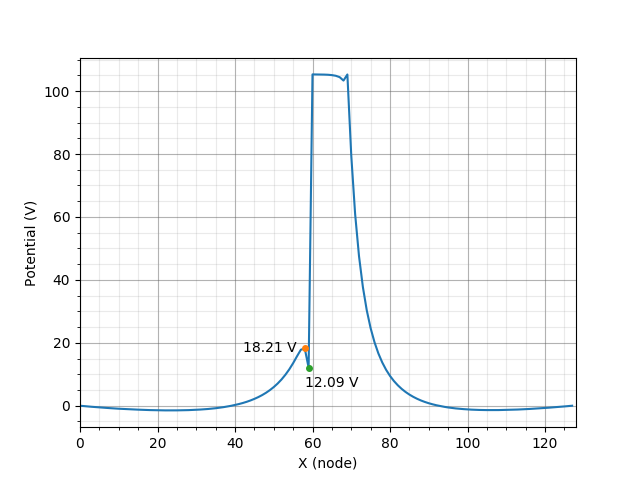
\includegraphics[width=\textwidth]{figures/MMO/minZ/WB/L_minZ_WB.png}
  \caption{Booms}
  \label{fig:L_minZ_WB}
\end{subfigure}
\begin{subfigure}[b]{0.6\textwidth}
  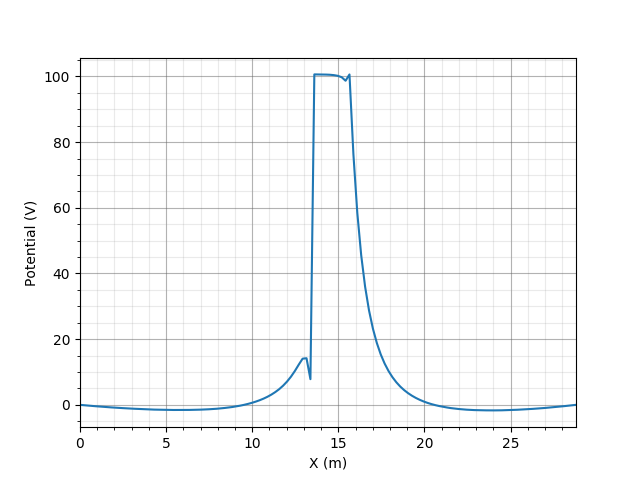
\includegraphics[width=\textwidth]{figures/MMO/minZ/NB/L_minZ_NB.png}
  \caption{Without booms}
  \label{fig:L_minZ_N}
\end{subfigure}
\label{fig:Line_minZ}
\caption{Potential profile along the X axis for the two MMO configurations with drift along the negative Z axis and photoemission included. The line is plotted at $(x,y) = (13.95 m, 13.95 m)$, or node points $(x,y) = (62,62)$, and passes through the main octagonal body of the spacecraft. The X axis units are in number of nodes from the origin. The two values in each plot show the height of the potential barrier formed.}
\end{figure}


%AVERAGE POTENTIAL ISOLINES XY
\begin{figure}[H]
  \begin{subfigure}[b]{0.6\textwidth}
    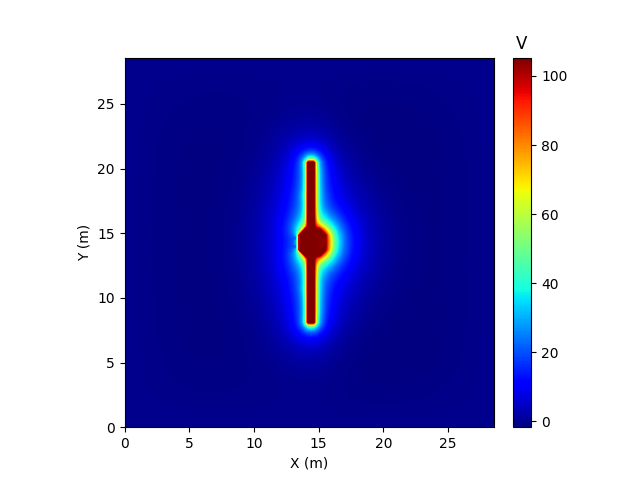
\includegraphics[width=\textwidth]{figures/MMO/minZ/WB/P_minZ_WB.png}
    \caption{Booms}
    \label{fig:P_minZ_WB}
  \end{subfigure}
  \hfill
  \begin{subfigure}[b]{0.6\textwidth}
    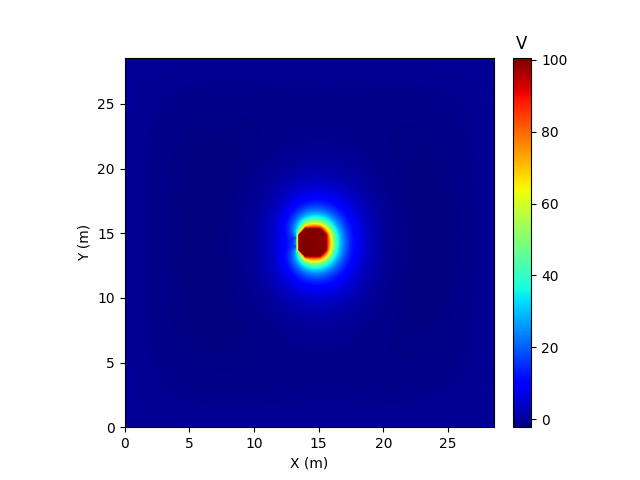
\includegraphics[width=\textwidth]{figures/MMO/minZ/NB/P_minZ_NB.png}
    \caption{Without booms}
    \label{fig:P_minZ_NB}
  \end{subfigure}
  \label{fig:Pot_minZ}
  \caption{2D slices through $Z = 14.4 m$ showing the time averaged potential profile of the entire computational domain with drift along the negative Z axis, and photoemission included. The potential is time averaged after a floating potential has been reached after 1,000 timesteps.}
\end{figure}

%PARTICLE DENSITIES (rho_i and rho_e)
%RHO_I
\begin{figure}[H]
  \begin{subfigure}[b]{0.6\textwidth}
  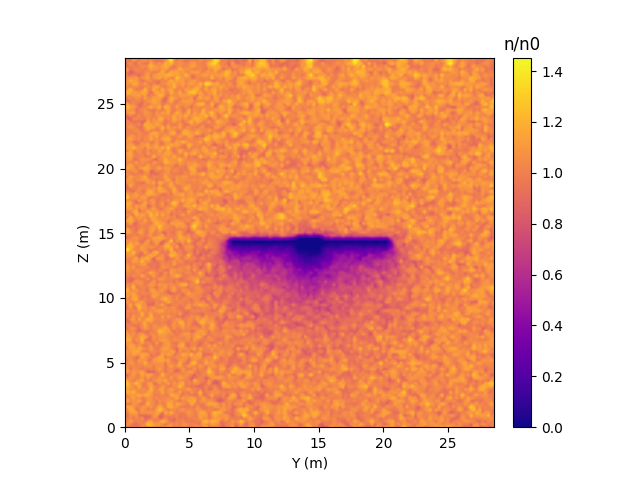
\includegraphics[width=\textwidth]{figures/MMO/minZ/WB/I_minZ_WB.png}
  \caption{Booms}
  \label{fig:I_minZ_WB}
\end{subfigure}
\begin{subfigure}[b]{0.6\textwidth}
  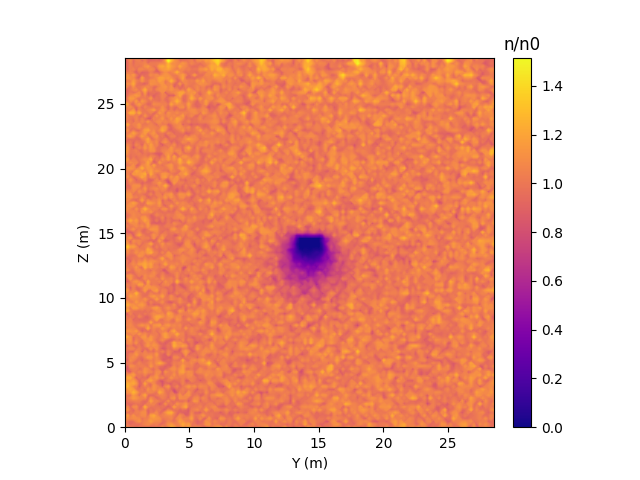
\includegraphics[width=\textwidth]{figures/MMO/minZ/NB/I_minZ_NB.png}
  \caption{Without booms}
  \label{fig:I_minZ_NB}
\end{subfigure}
\label{fig:Ion_minZ}
\caption{Ion density profile plotted at $Y = 14.4 m$, the color gradient is normalized against the ion plasma density from table \ref{tab:PlasmaParamMMO}. Drift is along the negative Z axis. and photoemission is included.}
\end{figure}

%RHO_E
\begin{figure}[H]
  \begin{subfigure}[b]{0.6\textwidth}
  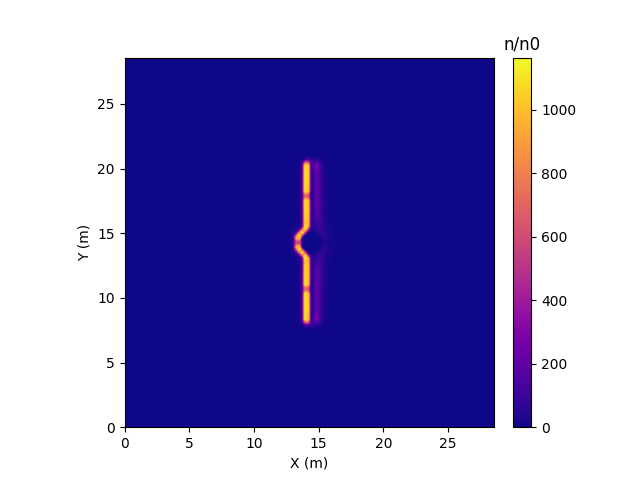
\includegraphics[width=\textwidth]{figures/MMO/minZ/WB/E_minZ_WB.png}
  \caption{Booms}
  \label{fig:E_minZ_WB}
\end{subfigure}
\begin{subfigure}[b]{0.6\textwidth}
  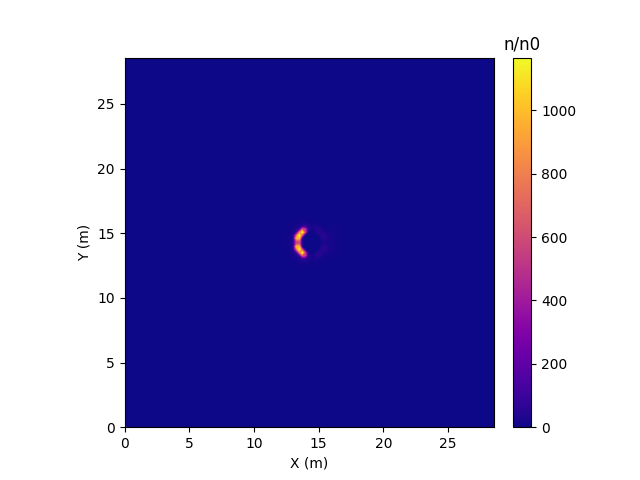
\includegraphics[width=\textwidth]{figures/MMO/minZ/NB/E_minZ_NB.png}
  \caption{Without booms}
  \label{fig:E_minZ_NB}
\end{subfigure}
\label{fig:Elec_minZ}
\caption{Electron density profile plotted at $Z = 14.4 m$, the color gradient is normalized against the electron plasma density from table \ref{tab:PlasmaParamMMO}. Drift is directed into the page, and photoemission is included. The sun is located in the negative X direction.}
\end{figure}


\section{Charging in an external magnetic field}

%FLOATING POTENTIAL CONVERGENCE
\begin{figure}[H]
  \begin{subfigure}[b]{0.75\textwidth}
  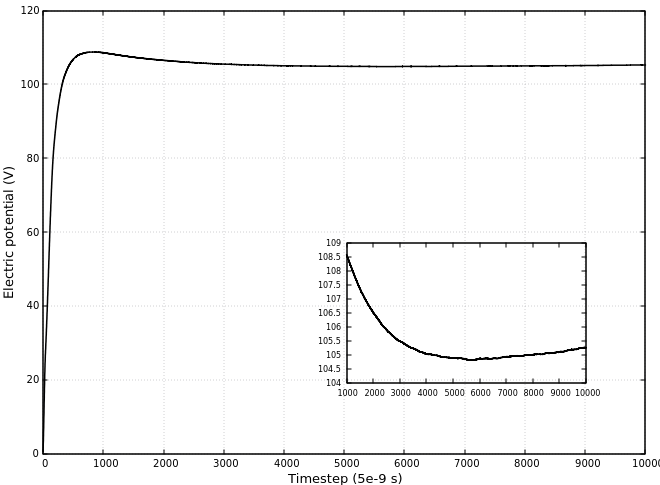
\includegraphics[width=\columnwidth]{figures/MMO/BField/WB/C_BField_WB.png}
  \caption{Booms}
  \label{fig:C_BField_WB}
\end{subfigure}
\par\bigskip
\begin{subfigure}[b]{0.75\textwidth}
  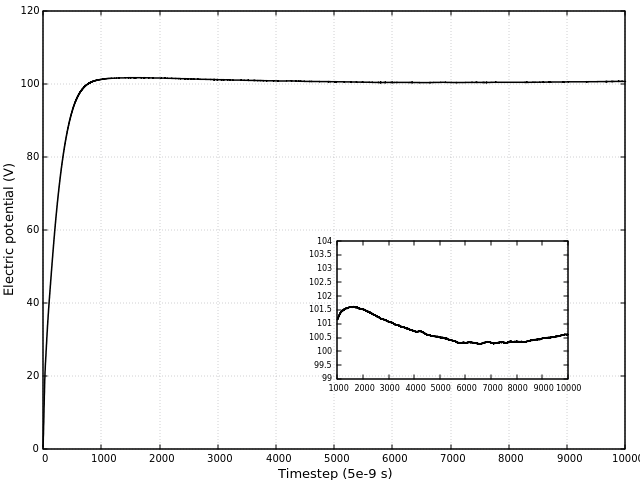
\includegraphics[width=\columnwidth]{figures/MMO/BField/NB/C_BField_NB.png}
  \caption{Without booms}
  \label{fig:C_BField_NB}
\end{subfigure}
\label{fig:Conv_BField}
\caption{Timeseries plot of the potential of the two configurations of the MMO, drift is along the negative Z axis, photoemission and an external magnetic field are included. The potential has been converted from PINC dimensionless units to Volts. The inset plots shows the potential of the two configurations for last 9,000 timesteps.}
\end{figure}


%POTENTIAL THROUGH CENTER OF OBJECT

\begin{figure}[H]
  \begin{subfigure}[b]{0.6\textwidth}
  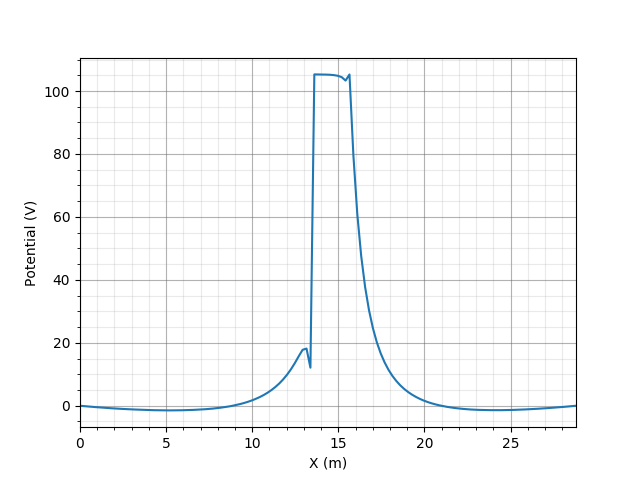
\includegraphics[width=\textwidth]{figures/MMO/BField/WB/L_BField_WB.png}
  \caption{Booms}
  \label{fig:L_BField_WB}
\end{subfigure}
\begin{subfigure}[b]{0.6\textwidth}
  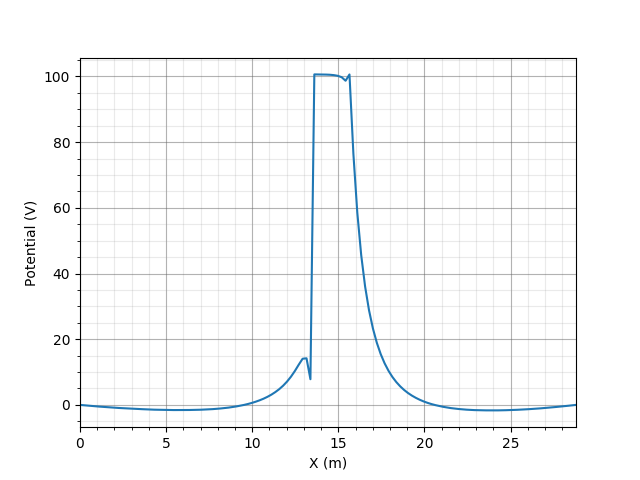
\includegraphics[width=\textwidth]{figures/MMO/BField/NB/L_BField_NB.png}
  \caption{Without booms}
  \label{fig:L_BField_NB}
\end{subfigure}
\label{fig:Line_BField}
\caption{Potential profile along the X axis for the two MMO configurations with drift along the negative Z axis, photoemission and an external magnetic field are included. The line is plotted at $(x,y) = (13.95 m, 13.95 m)$, or node points $(x,y) = (62,62)$, and passes through the main octagonal body of the spacecraft. The X axis units are in number of nodes from the origin. The two values in each plot show the height of the potential barrier formed.}
\end{figure}

%AVERAGE POTENTIAL ISOLINES XY
\begin{figure}[H]
  \begin{subfigure}[b]{0.6\textwidth}
    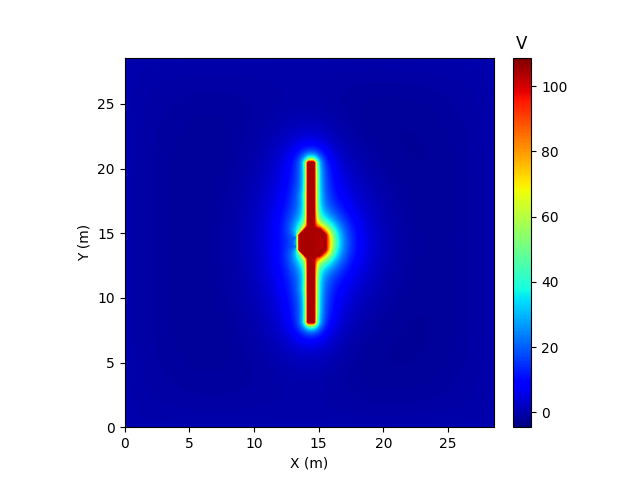
\includegraphics[width=\textwidth]{figures/MMO/BField/WB/P_BField_WB.png}
    \caption{Booms}
    \label{fig:P_BField_WB}
  \end{subfigure}
  \hfill
  \begin{subfigure}[b]{0.6\textwidth}
    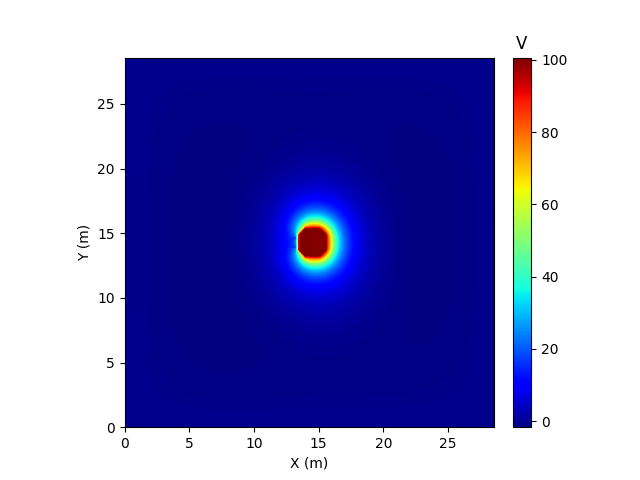
\includegraphics[width=\textwidth]{figures/MMO/BField/NB/P_BField_NB.png}
    \caption{Without booms}
    \label{fig:P_BField_NB}
  \end{subfigure}
  \label{fig:Pot_BField}
  \caption{2D slices through $Z = 14.4 m$ showing the time averaged potential profile of the entire computational domain with drift along the negative Z axis, photoemission and an external magnetic field are included. The potential is time averaged after a floating potential has been reached after 1,000 timesteps.}
\end{figure}

%PARTICLE DENSITIES (rho_i and rho_e)
%RHO_I
\begin{figure}[H]
  \begin{subfigure}[b]{0.6\textwidth}
  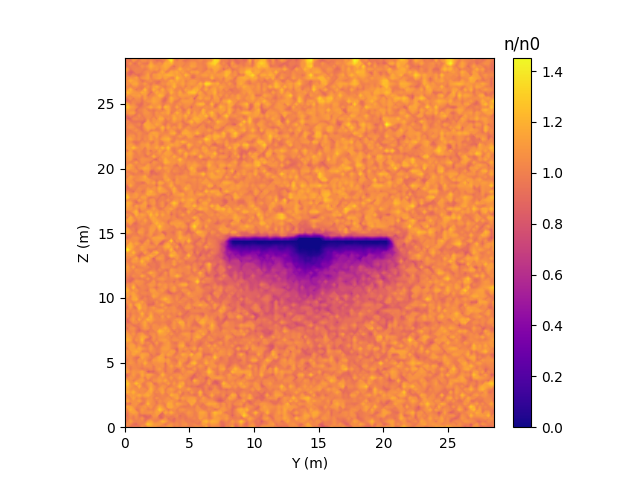
\includegraphics[width=\textwidth]{figures/MMO/BField/WB/I_BField_WB.png}
  \caption{Booms}
  \label{fig:I_BField_WB}
\end{subfigure}
\begin{subfigure}[b]{0.6\textwidth}
  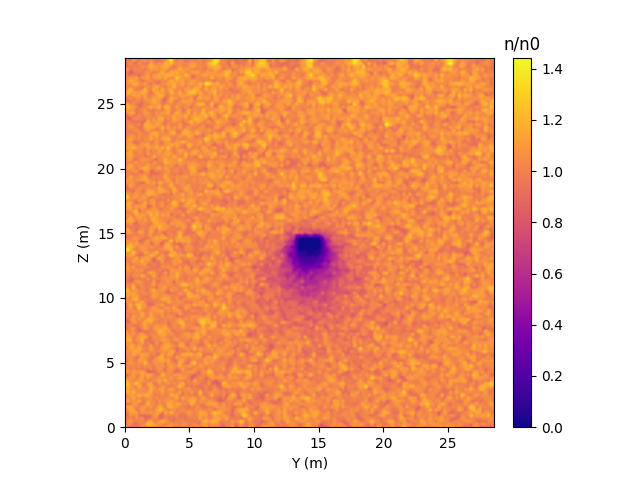
\includegraphics[width=\textwidth]{figures/MMO/BField/NB/I_BField_NB.png}
  \caption{Without booms}
  \label{fig:I_BField_NB}
\end{subfigure}
\label{fig:Ions_BField}
\caption{Ion density profile plotted at $Z = 14.4 m$, the color gradient is normalized against the ion plasma density from table \ref{tab:PlasmaParamMMO}. Drift is along the negative Z axis, photoemission and an external magnetic field are included.}
\end{figure}

%RHO_E
\begin{figure}[H]
  \begin{subfigure}[b]{0.6\textwidth}
  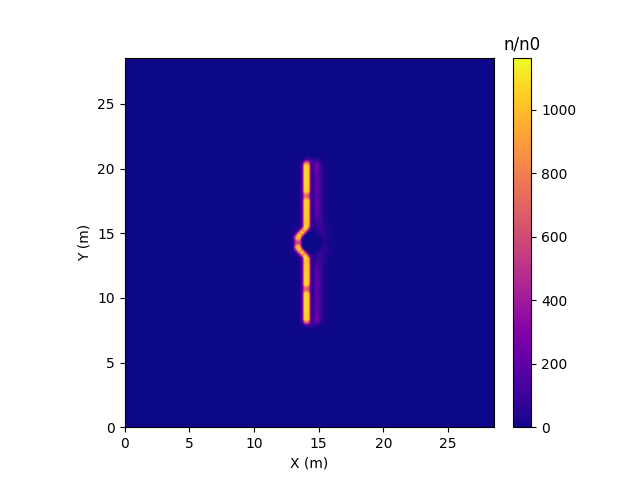
\includegraphics[width=\textwidth]{figures/MMO/BField/WB/E_BField_WB.png}
  \caption{Booms}
  \label{fig:E_BField_WB}
\end{subfigure}
\begin{subfigure}[b]{0.6\textwidth}
  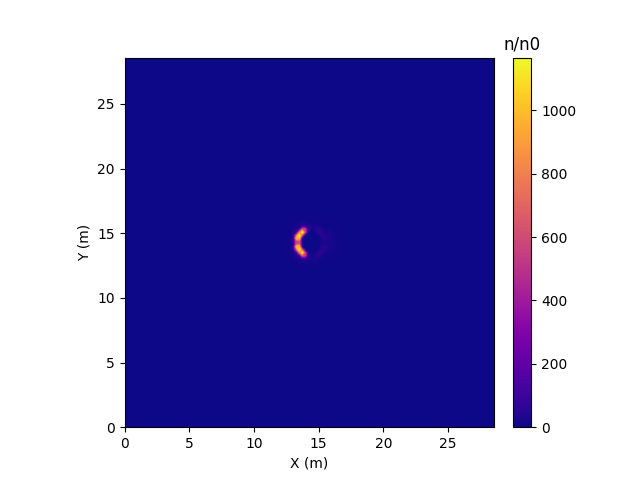
\includegraphics[width=\textwidth]{figures/MMO/BField/NB/E_BField_NB.png}
  \caption{Without booms}
  \label{fig:E_BField_NB}
\end{subfigure}
\label{fig:Elec_BField}
\caption{Electron density profile plotted at $Z = 14.4 m$, the color gradient is normalized against the electron plasma density from table \ref{tab:PlasmaParamMMO}.Drift is along the negative Z axis, photoemission and an external magnetic field are included. The direction of the sun is along the negative X axis.}
\end{figure}

\section{Charging at different photoelectron temperatures}

%FLOATING POTENTIAL CONVERGENCE
\begin{figure}[H]
  \centering
  \begin{subfigure}[b]{0.75\textwidth}
  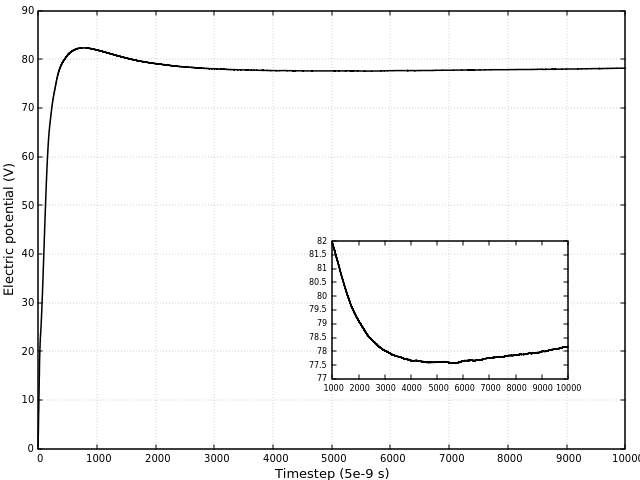
\includegraphics[width=\columnwidth]{figures/MMO/PHTemp/WB/C_PHTemp_WB.png}
  \caption{Booms}
  \label{fig:C_PHTemp_WB}
\end{subfigure}
\par\bigskip
\begin{subfigure}[b]{0.75\textwidth}
  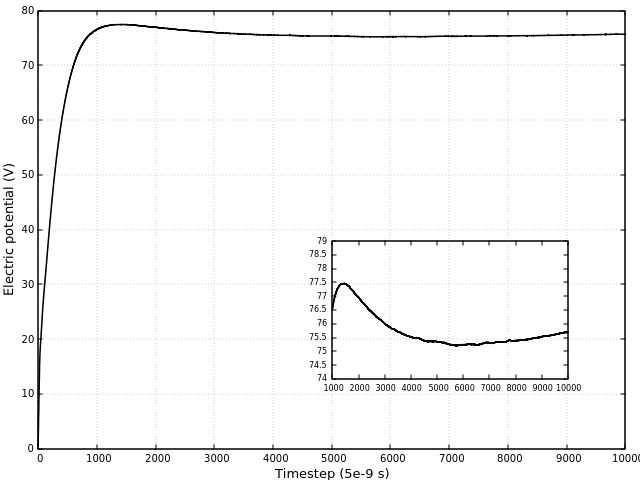
\includegraphics[width=\columnwidth]{figures/MMO/PHTemp/NB/C_PHTemp_NB.png}
  \caption{Without booms}
  \label{fig:C_PHTemp_NB}
\end{subfigure}
\label{fig:Conv_PHTemp}
\caption{Timeseries plot of the potential of the two configurations of the MMO, drift is along the negative Z axis and the photoelectron temperature has been set to $3 \; eV$. The potential has been converted from PINC dimensionless units to Volts. The inset plots the same timeseries after 1000 timesteps, where the potential of the spacecraft has begun to oscillate about the floating potential.}
\end{figure}

%POTENTIAL THROUGH CENTER OF OBJECT
\begin{figure}[H]
  \begin{subfigure}[b]{0.6\textwidth}
  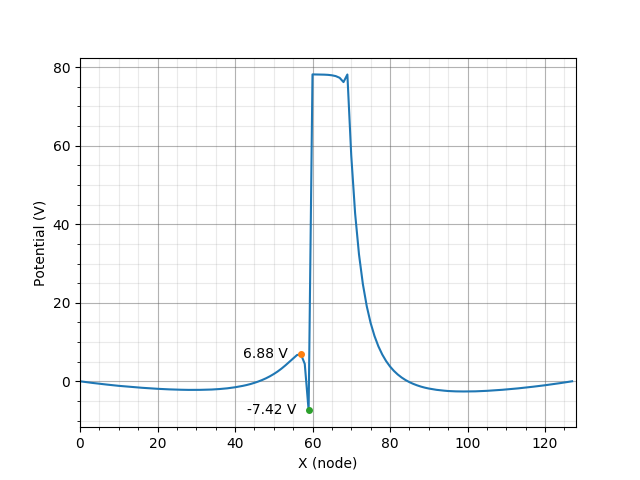
\includegraphics[width=\textwidth]{figures/MMO/PHTemp/WB/L_PHTemp_WB.png}
  \caption{Booms}
  \label{fig:L_PHTemp_WB}
\end{subfigure}
\begin{subfigure}[b]{0.6\textwidth}
  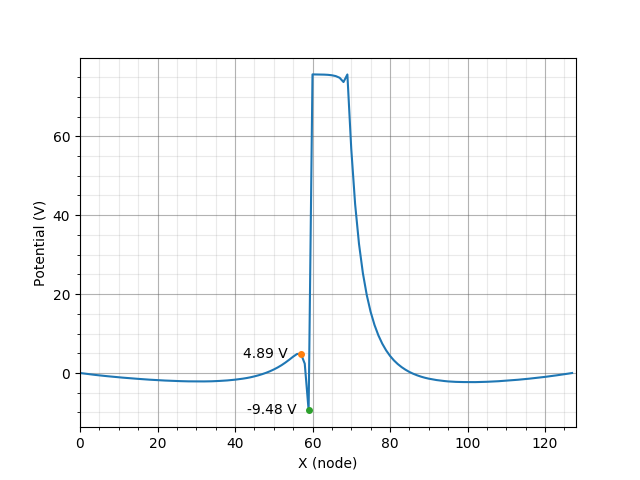
\includegraphics[width=\textwidth]{figures/MMO/PHTemp/NB/L_PHTemp_NB.png}
  \caption{Without booms}
  \label{fig:L_PHTemp_NB}
\end{subfigure}
\label{fig:Line_PHTemp}
\caption{Potential profile along the X axis for the two MMO configurations with drift along the negative Z axis, photoemission is included with a photoelectron temperature of $3 \; eV$. The line is plotted at $(x,y) = (13.95 m, 13.95 m)$, or node points $(x,y) = (62,62)$, and passes through the main octagonal body of the spacecraft. The X axis units are in number of nodes from the origin. The two values in each plot show the height of the potential barrier formed.}
\end{figure}

%AVERAGE POTENTIAL ISOLINES XY
\begin{figure}[H]
  \begin{subfigure}[b]{0.6\textwidth}
    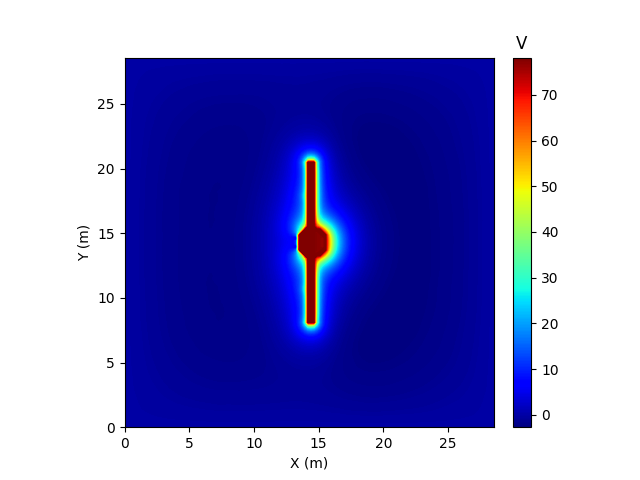
\includegraphics[width=\textwidth]{figures/MMO/PHTemp/WB/P_PHTemp_WB.png}
    \caption{Booms}
    \label{fig:P_PHTemp_WB}
  \end{subfigure}
  \hfill
  \begin{subfigure}[b]{0.6\textwidth}
    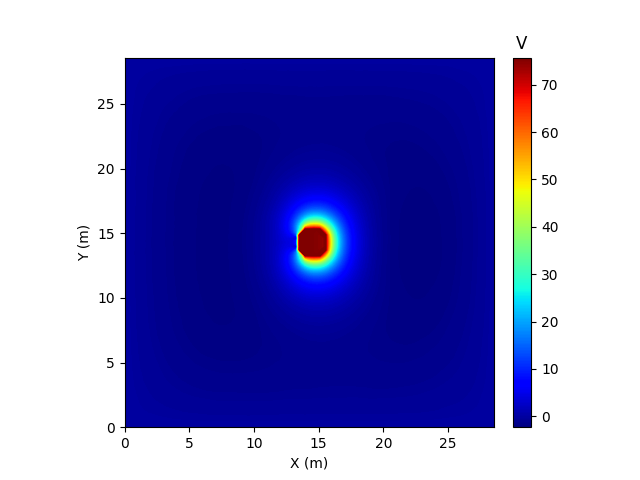
\includegraphics[width=\textwidth]{figures/MMO/PHTemp/NB/P_PHTemp_NB.png}
    \caption{Without booms}
    \label{fig:P_PHTemp_NB}
  \end{subfigure}
  \label{fig:Pot_PHTemp}
  \caption{2D cut through $Z = 14.4 m$ showing the time averaged potential profile of the entire computational domain with drift along the negative Z axis, photoemission is included with a photoelectron temperature of $3 \; eV$. The potential is time averaged after a floating potential has been reached after 1,000 timesteps.}
\end{figure}

%PARTICLE DENSITIES (rho_i and rho_e)
%RHO_I
\begin{figure}[H]
  \begin{subfigure}[b]{0.6\textwidth}
  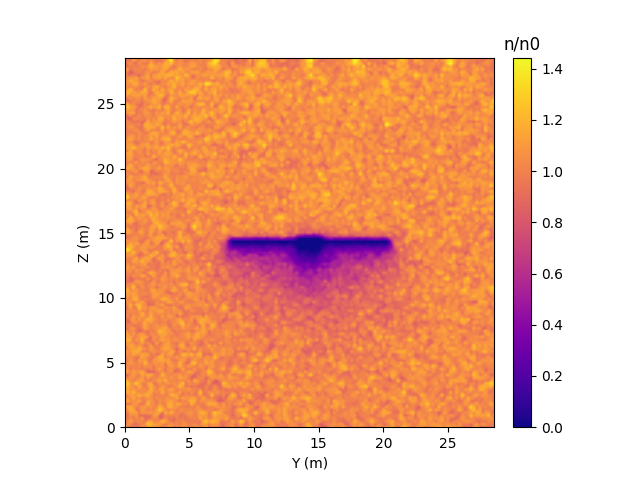
\includegraphics[width=\textwidth]{figures/MMO/PHTemp/WB/I_PHTemp_WB.png}
  \caption{Booms}
  \label{fig:I_PHTemp_WB}
\end{subfigure}
\begin{subfigure}[b]{0.6\textwidth}
  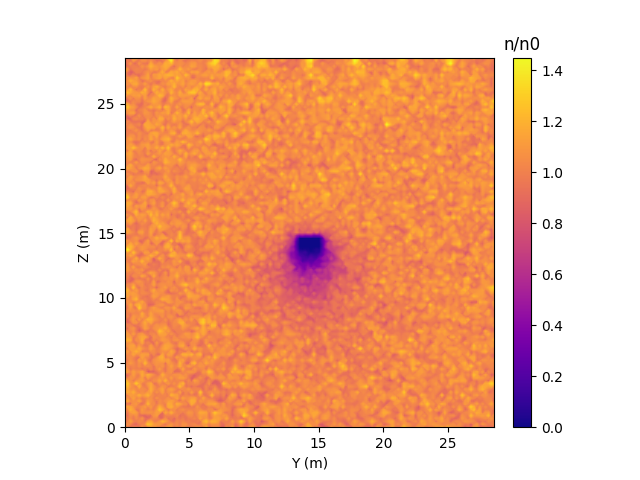
\includegraphics[width=\textwidth]{figures/MMO/PHTemp/NB/I_PHTemp_NB.png}
  \caption{Without booms}
  \label{fig:I_PHTemp_NB}
\end{subfigure}
\label{fig:Ions_PHTemp}
\caption{Ion density profile plotted at $Z = 14.4 m$, the color gradient is normalized against the ion plasma density from table \ref{tab:PlasmaParamMMO}. Drift is along the negative Z axis, and photoemission is included with a photoelectron temperature of $3 \; eV$.}
\end{figure}

%RHO_E
\begin{figure}[H]
  \begin{subfigure}[b]{0.6\textwidth}
  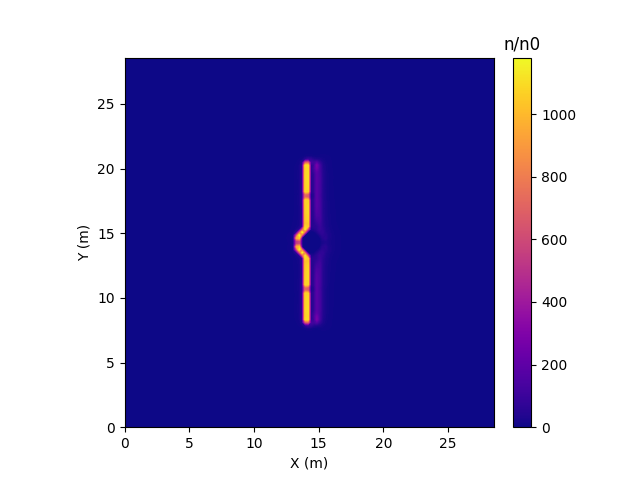
\includegraphics[width=\textwidth]{figures/MMO/PHTemp/WB/E_PHTemp_WB.png}
  \caption{Booms}
  \label{fig:E_PHTemp_WB}
\end{subfigure}
\begin{subfigure}[b]{0.6\textwidth}
  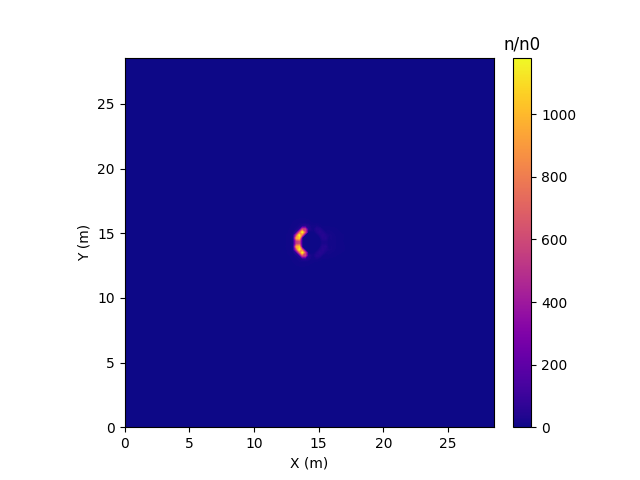
\includegraphics[width=\textwidth]{figures/MMO/PHTemp/NB/E_PHTemp_NB.png}
  \caption{Without booms}
  \label{fig:E_PHTemp_NB}
\end{subfigure}
\label{fig:Elec_PHTemp}
\caption{Electron density profile plotted at $Z = 14.4 m$, the color gradient is normalized against the electron plasma density from table \ref{tab:PlasmaParamMMO}. Drift is along the negative Z axis, and photoemission is included with a photoelectron temperature of $3 \; eV$.}
\end{figure}